
	\section{Многолучевая интерференция. Интерферометр Фабри-Перо. Формула Эйри.
		Пластинка Люммера-Герке. Интерференционные фильтры и зеркала. Просветление
		оптики.}
	\begin{figure}[h]
		\centering
		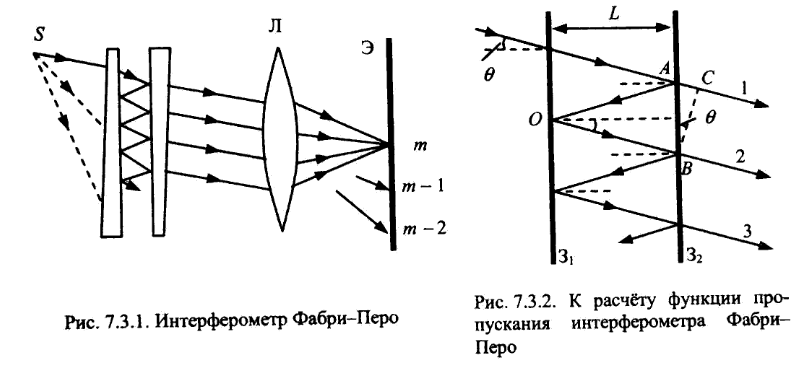
\includegraphics[scale = 0.7]{27_1}
	\end{figure}
	Интерферометр Фабри-Перо это два почти идеальных зеркала, которые отражают $\sim 99\%$ а оставшееся пропускают. Луч, попадая в нее испытывает многократные отражения. Обычно после интерферометра ставят линзу, что бы собрать параллельный пучек в точку.  Итак, пусть луч падает под углом $\theta$ на интерферометр. Надо думать, что он маленький, иначе не множественных отражений просто не будет. За один проход луч неберает фазу $\Delta = AOC - AB = \dfrac{2L}{\cos \theta} - 2L \tan \theta \sin \theta = 2L \cos \theta$ получается условие на максимумы будет иметь вид $2L \cos \theta = \lambda m$ \
	Пусть мы отражаемся много раз. Пусть на интерферометр падает луч с амплитудой $A$ и фазой ноль, тогда тот луч, который прошел ни разу не отразившись будет иметь $Ad^2$ тот который 2 раза отразился перед выходом $Ad^2 r^2 e^{i\delta}$  и так далее. Если угол тета мал, то отражений будет очень много, а $r^2 <1$ то просуммировав ряд получим:
	 \begin{align*}
	 A_{конечная} = Ad^2 \dfrac{1}{1 - r^2 e^{i\delta}}\\
	 \delta = 2L k\cos \theta\\
	 D = \dfrac{(1 - r^2)^2}{1 - 2r^2 \cos \delta + r^4}
	 \end{align*}
	 D это энергетический коэффициент пропускания. Так же это называется формулой Эйри, если судить по презентациям лектора.\\
	 \begin{figure}[t!]
	 	\centering
	 	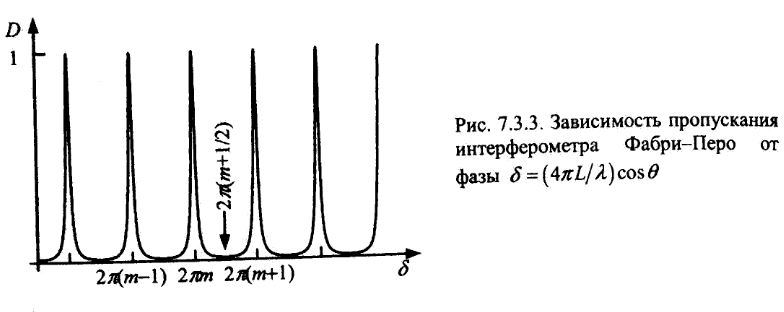
\includegraphics[scale = 0.5]{27_2}
	 \end{figure}
	 	Посмотрим на пластинку Люммера-Герке.
		\begin{figure}[h]
			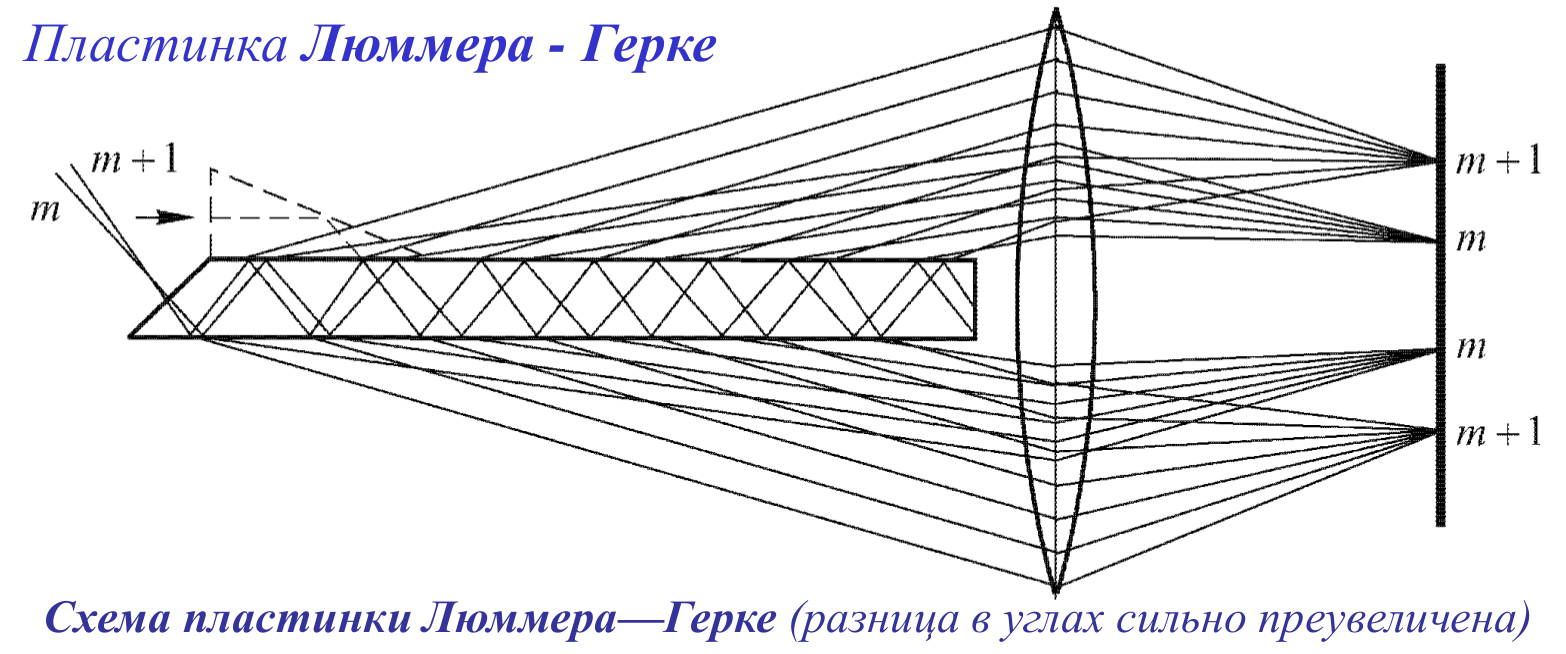
\includegraphics[scale = 0.3]{27_3}
		\end{figure}
		Что-то очень похожее на Фабри-Перо. Очевидно, что максимумы достигаются при условии $2d n \cos \theta = \lambda m$ где d толщина, а n- оптическая плотность \newpage
		\textbf{Просветление оптики}
		Допустим мы недовольны коэффициентом отражения стекла. Тогда мы можем нанести тонкий слой чего-нибудь на поверхность, главное чтобы это что-нибудь имело n меньше, чем у нашего стекла. При условии $\delta = \dfrac{2\pi}{\lambda} 2nh = (2m + 1)$ отраженная от первого края волна и отраженная от второго погасят друг друга и коэффициент прохождения увеличится.
		\begin{figure}[H]
			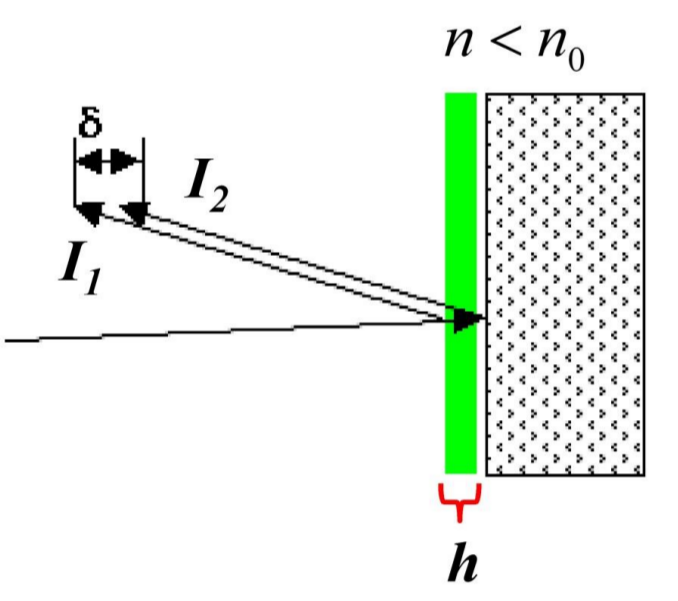
\includegraphics[scale = 0.3]{27_4}
		\end{figure}